\documentclass{tfg_domingo}
% \documentclass[numeros]{tfg_domingo}

\autor{Juan Toca Mateo}
\titulo{Secuencias binarias y sus aplicaciones}
% Título corto para los encabezamientos de pagina:
\corto{Binary sequences and their applications} % En blanco si no es necesario recortarlo.
\ingles{Binary sequences and their applications}
\fecha{septiembre de 2020}
% La normativa prescribe «cuatro o cinco palabras clave, en
% español y en inglés, para su indexación en el repositorio
% de TFG».
\palabras{secuencia, correlacion, señal}%
  {sequence, correlation, signal}

\usepackage{lipsum} % Esto solo es relleno.
\newcommand{\domingo}[1]{\textcolor{red}{#1}}
\begin{document}

% Si alguna palabra se divide entre dos líneas en un punto
% indebido, podemos indicar aquí los puntos de corte
% aceptables (si los hay), p. ej,
% \hyphenation{ba-rro-co, frío, cria-do, su-per-ra-tón}
\hyphenation{Dijkstra new-speak}

\portada
\frontmatter
% \sucinto{A Sofía}
\gracias{\input{Chapters/agradecimientos.txt}}
\resumen{El análisis de la correlación de señales es una pieza clave en múltiples
desarrollos de ingeniería tales como el GPS, el sónar o la corrección de errores
a la hora de transmitir información. Habiendo moldeado actividades tan diversas
como la conducción, la cartografía o el uso de internet, el estudio de la
función de autocorrelación puede derivar en nuevos desarrollos o mejoras en
los ya existentes. \\

En este proyecto, nos centramos en la generación de nuevas secuencias
pseudoaleatorias mas largas para, entre otros posibles usos, sonares y sistemas
GPS con mayor resolución. Para ello, se ha desarrollado un software desplegable
en un nodo de supercomputación para asistir en la búsqueda de dichas
secuencias.
}{The analisis of the correlation of signals is a key piece in several
engineering developments such as the GPS, the radar or the correction of errors
during information transmission. Having shaped so many diverse activities like
driving, cartography or internet usage, the study of the correlation function
may lead to new developments or improvements in the ones that already exist.\\

In this project, we focus on the generation of new pseudorandom sequences for
more accurate radars or GPS technologies. To do so, a new software, deployable
in a supercomputer, has been developed to assist in the search of these
sequences.
}
\tableofcontents

\mainmatter


\chapter{Introduction}

There is no doubt that signals have changed drastically the way we live.
Physical maps have passed out long ago in favor of real-time position tracking
systems. Who needs a meter when you can send a signal to measure distances
accuratly? Even publishing this project it's thanks to the hard work of
engineers that squeeze the capabilities of the carrier wave to transport
information throughout Internet. \\

In this chapter, we will introduce the correlation, autocorrelation and
crosscorrelation functions for periodic binary sequences and it's mathematical
properties. We will also take a look at pseudorandom noise, it's properties and
practical applications.


\section{Conventions}
 TODO

 %TODO: Add support for correlation with complex numbers

\section{Correlation function}

According to \citet{golomb_ref}, the correlation function measures how similar
two phenomena are. If properly normalized, the function ranges from
+1(identical) to -1(opposite); 0 meaning completly unrelated phenomena.
If we represent those phenomena as vectors, the correlation can be concived
as the normalized dot product between those 2 vectors.
In the discrete case where both sequences have the same length (the one we are
going to focus on), the normalized version is defined as follows:

\begin{definition}[Normalized correlation]\label{def:1}

Given $\alpha$ and $\beta$ two vectors of the same length n and $\alpha_{i}$
and $\beta_{i}$ the components of the vectors:

\begin{equation}\label{eq:1}
C(\alpha , \beta)=\frac{(\alpha \cdot  \beta)}{|\alpha||\beta|}=\frac{\sum_{i=1}^{n} \alpha_{i}\beta_{i}}{(\sum_{i=1}^{n} \alpha_{i}^{2})^{\frac{1}{2}}(\sum_{i=1}^{n} \beta_{i}^{2})^\frac{1}{2}}
\end{equation}
\end{definition}

Notice that in this vector
representation:
\begin{itemize}
  \item Orthogonal vectors have a correlation value of 0
  \item Vectors with the same direction and orientation have a correlation
  value of 1
  \item Vectors with the same direction but opposite orientation have a
  correlation value of -1
\end{itemize}

Even though the normalized version is the best way to represent the degree
of similarity between 2 phenomena and a good way to grasp the concept of
what we are defining, for the rest of the document we are going to use the
unnormalized version if not specified. This version of the correlation function
have several advantages for our research as it is simpler and carries the same
amount of information, saving us some computation resources and complexity on
our theoretical analysis. Keep in mind that it's always posible to move from
applied to the normalized one if we need it. The unnormalized correlation is
defined as:

\begin{definition}[Unnormalized correlation]\label{def:2}
  Given $\alpha$ and $\beta$ two vectors of the same length n and $\alpha_{i}$
  and $\beta_{i}$ the components of the vectors:
  \begin{equation}\label{eq:2}
    C(\alpha , \beta) = (\alpha \cdot  \beta) = \sum_{i=1}^n(\alpha \odot \beta)_{i}= \sum_{i=1}^{n} \alpha_{i}\beta_{i}
  \end{equation}

  Where "$\odot$" represents the pointwise product of vectors.

\end{definition}

Adapting this function from vectors to finite digital signals is straight
forward, as they can be defined in terms of a vector that lives in a vector
space of dimension equal to the length of the signal.


\begin{figure}[ht!] % [h!] fuerza que el elemento se sitúe
                    % en la posición señalada, en vez de al
                    % comienzo de una página.
\begin{center}
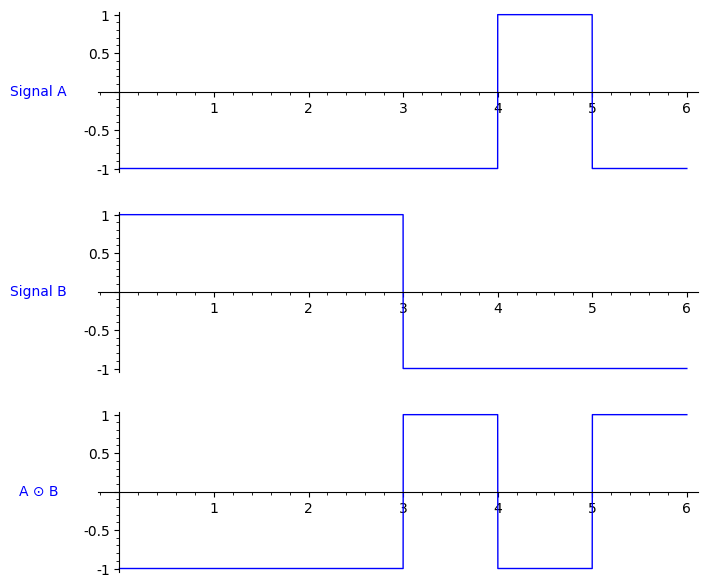
\includegraphics[width=0.7\linewidth]{Chapters/Introduction/signals_correlation}
\end{center}
\caption{Representation of 2 signals an their pointwise product with an unnormalized correlation between them of -2(-1 -1 -1 +1 -1 +1)}
\label{introduction_signals_hadamard}
\end{figure}

If we take a look at Figure \ref{introduction_signals_hadamard}, we can see
a simple computation that can easily be implemented in a chip. Notice that,
in contrast of what would be needed for the normalized version, we only use
integer arithmetics, multiplication and addition rather than squaring along the
signal proccesing and then calculating the square root.











\section{Autocorrelation function}

Going on with the lecture of \citet{golomb_ref}, the autocorrelation function
is a measure of how the correlation behaves if, for a given sequence, a
circular shift is applied and correlated with the original sequence for every
possible shift. It is defined for periodic sequences as follows:

\begin{definition}[Autocorrelation]\label{def:3}

Given the function C defined in Equation \ref{eq:2} and n the length of the
sequence S

\begin{equation}\label{eq:3}
  shift(S, \tau)_i = S_{(i+\tau) \bmod n}
\end{equation}
\begin{equation}\label{eq:4}
  A(S)_{\tau} = C(S, shift(S, \tau)) = \sum_{i=1}^{n}S_{i}S_{(i+\tau) \bmod n}
\end{equation}

\end{definition}

\begin{figure}[ht!] % [h!] fuerza que el elemento se sitúe
                    % en la posición señalada, en vez de al
                    % comienzo de una página.
\begin{center}
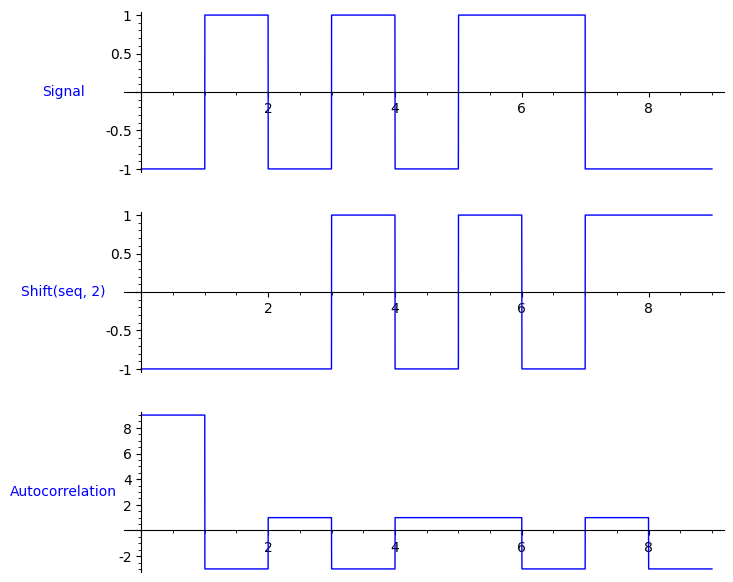
\includegraphics[width=0.7\linewidth]{Chapters/Introduction/signals_autocorrelation}
\end{center}
\caption{A signal with a shifted version of itself and it's autocorrelation function}
\label{introduction_signals_autocorrelation}
\end{figure}

An example of this function is shown in Figure
\ref{introduction_signals_autocorrelation} in which we can find examples of
some important properties of the autocorrelation function:

\begin{theorem}\label{theorem:1.2.1}
  Given a sequence S, the autocorrelation value for $\tau = 1$ is:
    \begin{equation}
      A(S)_{1}=C(S, S)=\sum_{i=1}^{n}S_{i}^2
    \end{equation}
\end{theorem}

\begin{corollary}
  Given the unnormalized autocorrelation of a sequence, we can
  normalize it by dividing it as follows:
  \begin{equation}
    A'(S)_{\tau} = \frac{A(S)_{\tau}}{A(S)_{1}}
  \end{equation}
\end{corollary}

\begin{proof}
  Using Equations \ref{eq:1} and \ref{eq:4}, we can normalize \ref{eq:4} as
  follows:

    $$A'(S)_{\tau} = C'(S, shift(S, \tau)) = \frac{C(S, shift(S, \tau))}{(\sum_{i=1}^{n} S_{i}^{2})^{\frac{1}{2}}(\sum_{i=1}^{n} S_{i+\tau}^{2})^\frac{1}{2}} = \frac{A(S)_{\tau}}{\sum_{i=1}^{n} S_{i}^{2}} = \frac{A(S)_{\tau}}{A(S)_{1}}$$

  Keep in mind that, even though $S_{i}^2$ and $S_{i+\tau}^2$ aren't the same element, the elements of the shifted version are the same as the original sequence so the total sum is the same.
\end{proof}

\begin{corollary}\label{autocorrelation:coro:1}
  Given the autocorrelation of a sequence, $A_{1}(S)$ will always be the maximum value of the autocorrelation.
\end{corollary}

\begin{property}
 Components of the autocorrelation vector belong to the same group as the
  original sequence.
\end{property}

Even though this seems a naive property, this will prove
useful when we introduce the algorithm based in the Fourier Transform to
compute the autocorrelation function.









\section{Crosscorrelation function}

The crosscorrelation function measures how a sequence correlates with all
the posible shifts of another sequence. This function is useful in signal
proccesing to analyze if two signals can be mistaken one for another by a
receiver.


\begin{definition}[Crosscorrelation]\label{def:4}
  Given C the correlation function defined in Equation \ref{eq:2}, shift as the function defined in Equation \ref{eq:3} and n the length of both sequences:
  \begin{equation}\label{eq:7}
    CC(S1, S2)_{\tau} = C(S1, shift(S2, \tau)) = \sum_{i=1}^{n}S1_{i}S2_{(i+\tau) \bmod n}
  \end{equation}
\end{definition}

\begin{figure}[ht!] % [h!] fuerza que el elemento se sitúe
                    % en la posición señalada, en vez de al
                    % comienzo de una página.
\begin{center}
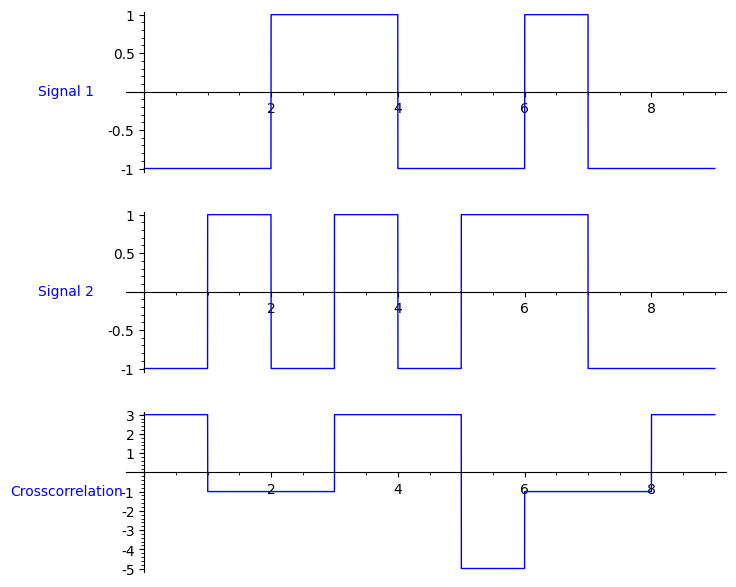
\includegraphics[width=0.7\linewidth]{Chapters/Introduction/signals_crosscorrelation}
\end{center}
\caption{Two signals and it's crosscorrelation}
\label{introduction_signals_crosscorrelation}
\end{figure}

\begin{lemma}\label{lem:1}
  Given a sequence S, CC the crosscorrelation function defined in Equation
  \ref{eq:7} and A the autocorrelation function defined in Equation \ref{eq:4}:
  \begin{equation}\label{eq:8}
    CC(S, S) = A(S)
  \end{equation}
\end{lemma}












\section{Pseudorandom noise(PRN)}

Noise have a different meaning depending on the field of study in which is
used. In our case we are going to work with random vectors of white noise,
which is defined as vectors in which all the components are statistically
independent between them.\cite{white_noise}\\

Even though noise in general is usually seen as an unwanted wave that
limits the amount of information that can be transmited through a
channel\cite{shannon_noise}, it has some practical uses:


\begin{outline}
  \1 PRN-based radars\cite{prn_radar_example1}\cite{prn_radar_example2}
  \1 As the spreading code in direct-sequence spread spectrum(DSSS) \cite{DSSS_1}\cite{DSSS}
    \2 CDMA in wireless communication\cite{DSSS}
    \2 GPS\cite{GPS}
\end{outline}

This practical applications exploit an important noise property:

\begin{property}
  The autocorrelation of a vector of white noise equals 0 for every component
  where $\tau \neq 1$ \cite{everett}
\end{property}

Taking a radar as an example, using this theorem can compute the distance
just by sending a white noise signal to a target and start correlating the
received signal with the original one. As the autocorrelation of
white noise only has a spike when the shift is 0, that spike represents in
which time instant the signal has returned. With that time instant, we can
get the round-trip time and then the actual distance if we know the
propagation speed of the wave.\\

In the case of GPS, the restrictions imposed to the noise sequence are
stronger. First of all, as we will be transmiting several signals in the same
frecuency, we need a set of codes with good crosscorrelation properties
between them. In other words, the crosscorrelation function between two given
codes must trend to 0 in every component, except when $\tau = 1$ and
both codes are the same.\\

As noise is an statistical construct, noise measured from natural phenomena
can generate sequences with poor correlation properties. As both technologies
depend on this properties to work, we must find a way of creating sequences
with properties similar to those of noise in an deterministic and efficient
fashion.\\

This kind of sequences are called Pseudorandom Noise(PRN). In practical
applications, PRN sequences aren't perfect noise because generating it is
difficult and unnecesary. In reality, we don't need an actual 0 in every
position of the autocorrelation. If we let the sequence take values in a
threshold so that the system won't mistake intermidiate values with the
autocorrelation spike, it will behave as expected.

\begin{figure}[ht!] % [h!] fuerza que el elemento se sitúe
                    % en la posición señalada, en vez de al
                    % comienzo de una página.
\begin{center}
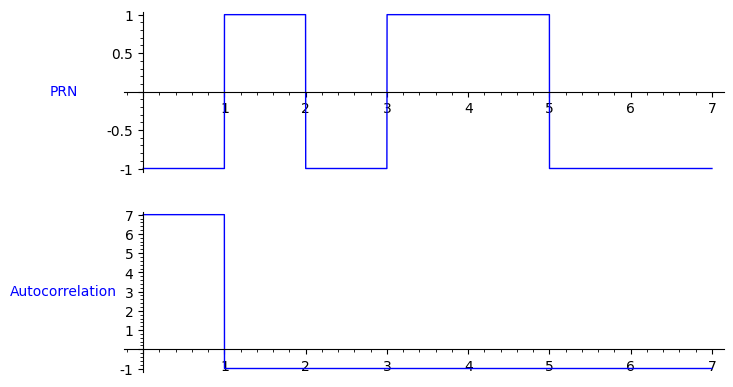
\includegraphics[width=0.7\linewidth]{Chapters/Introduction/signals_prn}
\end{center}
\caption{A pseudorandom noise sequence an it's autocorrelation function.
Notice that this PRN code isn't perfect noise.}
\label{introduction_signals_autocorrelation}
\end{figure}

% TODO Define family of sequences

% TODO Define flat autocorrelation



\chapter{PRN generation}

As explained in the previous chapter, pseudonoise sequences are useful in
tecnologies that need properties similar to those of white noise. In this
chapter, some state-of-the-art tecniques in pseudonoise generation
will be introduced.

\section{Maximum Length Sequence(m-sequences)}

M-sequences are an exponential binary pseudonoise construction that was
initially concived using linear feedback shift registers(LFSR). The particular
type of LFSR used in m-sequences can be simulated with extensions of binary
Finite Fields. The definitions are:

\begin{definition}[LFSR]
  A m-sequence is a binary sequence generated by an LFSR that, given an initial
  state different from 0, it cycles between all posible states except 0.
\end{definition}

Which, as shown in \citet{golomb_ref}, is equivalent to:

\begin{definition}[Finite Fields]
  Given $E/GF(2)$, $\alpha$ a primitive element of $E$ and $S$ the resulting
  sequence:
  \begin{equation}
    S_{i} = trace(\alpha^{i})
  \end{equation}
\end{definition}

\begin{property}
  A m-sequence will always be of length of the form $2^{n}-1$ where n is an
  arbitrary natural number.
\end{property}

\begin{property}
  A m-sequence sequence will always have an autocorrelation function such as
  all the components will be -1 except when $\tau = 1$
\end{property}

\begin{figure}[ht!]
  \inputpython{Chapters/PRN_generation/example_mls.py}{0}{100}
  \caption{An example of a posible implementation of m-sequences}
  \label{mls:fig:1}
\end{figure}

Notice that, even though the construction is exponential, the complexity of
the algorithm is $O(n)$ when $n$ is the size of the sequence. The problem is
that sequences of arbitrary size might be needed in some applications. As it will
be discussed see in a following chapter, the complexity of computing the
autocorrelation with the Fourier Transform approach is $O(n*log(n))$ so using longer
sequences than needed has a direct impact on the performance of the system. \\

This sequences by themselves might not a be huge deal because they don't define
a way to build families of well crosscorrelated sequences, but they are the
building blocks for other contructions, such as the Gold Codes used in GPS and
CDMA.

\section{Gold Codes}

Gold codes\cite{gold_codes} are a family of sequences, derived from
m-sequences, with very important properties that are used in several
applications such as wireless communication and geolocalisation. A Gold Code
generator gets two m-sequences sequences that fulfill:

\begin{property}
  Given two m-sequences that can generate Gold Codes, $S1$ and $S2$, of length
  $2^{n}-1$, $CC$ the crosscorrelation function defined in Equation \ref{eq:7}:
    \begin{equation}\label{gold:eq:1}
      max |CC(S1, S2)| \leq 2^{\frac{n+2}{2}}
    \end{equation}
\end{property}

And XORs all their relative shifts generating a family of $2^{n} + 1$ sequences
($2^{n} - 1$ XORed sequences + 2 m-sequences).

\begin{property}
  Given any two sequences, S1 and S2, from a Gold family of sequences of length
  $2^{n}-1$, $CC$ the crosscorrelation function defined in Equation \ref{eq:7}:
  \begin{equation}
        max |CC(S1, S2)| \leq \left\{\begin{array}{lr}
            2^{\frac{n+2}{2}}+1 & \textnormal{ if n is even } \\
            2^{\frac{n+1}{2}}+1 & \textnormal{ if n is odd } \\
        \end{array}\right.
  \end{equation}
\end{property}

% TODO: Add a  code example

This property means that the crosscorrelation between any given pair of
sequences from a Gold family is low enough to differentiate them. This proves
useful when several devices are transmiting in the same frecuency and we must
treat signals that are not the one we want to receive as noise.\\

Gold also showed  a way to generate this pair of sequences,
using a decimation of one m-sequence.

\begin{definition}[Decimation]
  Given a sequence $S$ of length $n$, a decimation by $q$ of $S$ is defined as:
  \begin{equation}
    S[q]_{i} = S_{((q·i) \bmod n)}
  \end{equation}
\end{definition}

\begin{property}
  Given a m-sequence $S$ of length $2^n - 1$ where n is odd and and a
  coprime of $n$ named $k$, the sequence pair $(S, S[2^{k} + 1])$ number
  fulfills equation \ref{gold:eq:1}.
\end{property}

\begin{figure}[ht!]
  \inputpython{Chapters/PRN_generation/example_gold.py}{0}{100}
  \caption{An example implementation of a generation of a family of gold
  sequences relying in the example at Figure \ref{mls:fig:1}.}
  \label{}
\end{figure}

Notice that this construction has the same problem as m-sequences. It's
an exponential contruction so it might not be enough for some applications.

\section{Legendre sequences}

Legendre sequences, as explained in \citet{legendre_sequences}, are binary
sequences defined through quadratic residues as follows:

\begin{definition}
  Let $p$ be an odd prime and the function "Legendre Symbol" be:
    \begin{equation}
      LSy(n, p) = \left\{\begin{array}{lr}
          1  & \textnormal{if n is a quadratic residue mod p}   \\
          -1 & \textnormal{otherwise} \\
      \end{array}\right.
    \end{equation}
  We define the Legendre Sequence as:
    \begin{equation}
      LSs(p)_{i} = LSy(i-1, p) \textnormal{  where  } 1 < i \leq p
    \end{equation}
\end{definition}

\begin{figure}[ht!]
  \inputpython{Chapters/PRN_generation/example_legendre.py}{0}{100}
  \caption{An example implementation of the generation of a Legendre sequence.}
  \label{}
\end{figure}

Some Legendre Sequences have interesting autocorrelation properties:
\begin{property}\label{property:2.3.1}
  Given an odd prime $p$ such as $p \equiv 3 \bmod 4$, we can say that
  $LSs(p)$ has a flat autocorrelation.\cite{legendre_sequences}
\end{property}

Even though \citet{legendre_sequences} has a generalization of property
\ref{property:2.3.1} to all Legendre Sequences, it requires the introduction of
a third symbol making the sequence non-binary. \\

As $p$ is the variable defining the size of the generated sequence, we can
derive that the distribution of Legendre Sequences is related to the Prime
Number Theorem. This means that Legendre Sequences have more possible lengths
than in m-sequences or other exponential contructions. However, Legendre
Sequences have the drawback that there is only one per sequence length.

\section{Composition method}

\subsection{Algorythm}

The composition method uses a base sequence and a sequence of shifts to
create a matrix of sequence components as follows:

\begin{definition}[Composite matrix]
  Given a base sequence $S$ of length $n$ and a sequence of integers $T$ of
  length $m$ such that:
  \begin{equation}\label{composition:eq:1}
    0 \leq T_{i} < n
  \end{equation}
  \begin{equation}\label{composition:eq:2}
    gcd(n, m) = 1
  \end{equation}

  Given the $shift$ function defined in Equation \ref{eq:3},
  we define the composite matrix as:

  \begin{equation}\label{composition:eq:3}
    CM(S, T) = \begin{bmatrix}
      shift(S, T_{0})_{0} & shift(S, T_{1})_{0} & \dots & shift(S, T_{m-1})_{0} \\
      shift(S, T_{0})_{1} & shift(S, T_{1})_{1} \\
      \vdots & & \ddots \\
      shift(S, T_{0})_{n-1} & & & shift(S, T_{m-1})_{n-1}
    \end{bmatrix}
  \end{equation}

  In other words, each column represents a shift of the base sequence defined
  by the sequence of shifts.
\end{definition}

\begin{definition}[Composite sequence]
  Given a base sequence $S$ of length $n$ and a sequence of integers $T$ of
  length $m$ that fulfill Equations \ref{composition:eq:1} and
  \ref{composition:eq:2} and the composite matrix defined at Equation
  \ref{composition:eq:3}, we define the composite sequence as:
  \begin{equation}
    CS(S, T)_{i} = CM(S, T)_{(i \bmod m), (i \bmod n)}
  \end{equation}
\end{definition}

\begin{figure}[ht!]
  $$S = \begin{bmatrix}
    0 & 1 & 2 & 3 & 4\\
  \end{bmatrix}$$
  $$T = \begin{bmatrix}
    0 & 2 & 1 & 4 & 3 \\
  \end{bmatrix}
  $$
  $$CM(S, T) = \begin{bmatrix}
  0 & 3 & 4 & 1 & 2 & 4\\
  1 & 4 & 0 & 2 & 3 & 0\\
  2 & 0 & 1 & 3 & 4 & 1\\
  3 & 1 & 2 & 4 & 0 & 2\\
  4 & 2 & 3 & 0 & 1 & 3\\
  \end{bmatrix}
  $$
  $$CS(S, T) = \text{[0 4 1 4 1 4 1 0 2 0 2 0 2 1 3 1 3 1 3 2 4 2 4 2 4 3 0 3 0 3]}\\
  $$
  \caption{Example of a computation of the composition method(note that we are
  using a non-binary sequence to illustrate better the method)}
  \label{}
\end{figure}

\subsection{Costas arrays}

Costas arrays, discovered independently by John P. Costas\cite{costas_costas}
and E.N. Gilbert \cite{gilbert_costas} in 1965, are a set of sequences highly
used in radar and sonar applications. We are going to provide the 2 definitions
as both will be useful for different purposes:

\begin{definition}[Costas array(Costas)]
  Square matrix of size $n×n$ filled with 0s and 1s such that there
  aren't more than multiple 1s in each row or column and that every
  displacement vector is distinct from the rest.
\end{definition}

This definition is used in several deployments of sonar and radar to generate
systems with a good ambiguity function, in other words, tolerant to Doppler
effect.

\begin{figure}[ht!]
  $$
  \begin{bmatrix}
   1&0&0&0\\
   0&0&0&1\\
   0&1&0&0\\
   0&0&1&0
  \end{bmatrix}
  $$
  \caption{An example of a Costas array}
  \label{fig:costas_1}
\end{figure}

Notice that we could compact the representation by just having a list of the
rows in which each 1 lives:

\begin{figure}[ht!]
  $$[4, 2, 1, 3]$$
  \caption{The compact representation of the Costas array of Figure
  \ref{fig:costas_1}}
  \label{fig:costas_2}
\end{figure}

This representation is equivalent to the definition of a Costas array provided
by Gilbert:

\begin{definition}[Distinct difference permutations]\label{def:costas_1}
  Given a sequence of integers $S$ of length $n$ such that:
    \begin{equation}\label{eq:costas_1}
      0 \leq S_{i} < n
    \end{equation}
  We say that $S$ is a distinct difference permutation $r$ apart if,
  for any given pair $(S_{i}, S_{j})$, satisfies:
    \begin{equation}\label{eq:costas_2}
      S_{i} - S_{i+r} \not \equiv S_{j} - S_{j+r} \bmod n
    \end{equation}
\end{definition}

\begin{definition}[Costas array(Gilbert)]
  Given a sequence $S$ satisfying Equation \ref{eq:costas_1}, we say it's a
  Costas array if, for any given $r$ value, it satisfies Equation
  \ref{eq:costas_2}.
\end{definition}

This compact representation can be feeded into the composition method as
a sequence of shifts generating interesting new sequences. [citation needed]\\

Several construction methods have
been proposed. For sake of simplicity, we are going to introduce just the Welsh
construction as defined in Gilbert \cite{gilbert_costas}:\\

Given a prime number $p$ and a primitive root $g$ of $p$, we can contruct a
Costas array $S$ as follows:
\begin{equation}
  S_{i} \equiv g^{i} \bmod p
\end{equation}

Notice that this contruction can generate sequences of a prime length as in
the Legendre Sequences. However, it can generate several sequences for a given
length. As the number of possible sequences depend on the number of primitive
elements of the finite field of order $p$, the number of possible costas arrays
for a given length using this construction is $\phi(p-1)$ where $\phi$ is the
Euler's totient function.



\chapter{Exhaustive search of binary sequences}
  \section{Previous work}

  As shown in the previous chapter, algebraic constructions for sequences
  with  low off-peak autocorrelation have huge constraints on the length of
  the generated sequences. To overcome this limitation, exhaustive searches
  through all possible candidates for a given length have been conducted in the past. The size of the search space in this case is  $O(2^n)$, where $n$ is the length of the binary sequence, which make their
 results very costly in terms of computational complexity.\\

For a similar case there has been studies for finding sequences with low aperiodic autocorrelation, whereas fewer works has been done in the periodic autocorrelation due to the existance of the optimal algebraic constructions, which have been sufficient for past practical purposes. In the next paragraphs  we review the literature on the aperiodic autocorrelation.\\

 First of all, aperiodic autocorrelation  and the energy of a sequence  are defined as follows.\\
  \begin{definition}[Aperiodic autocorrelation]
      Given a binary sequence $S$, its aperiodic autocorrelation is defined as:
      \begin{equation}
        A'_{\tau}(S) = \sum_{i=0}^{n-\tau-1}s_{i}s_{i+\tau}
      \end{equation}
  \end{definition}

  \begin{definition} Given a binary sequence $S$, the energy of $S$ is defined
    as:
    \begin{equation}
      E(S) = \sum_{k=1}^{n-1} A'_{k}(S)^{2}
    \end{equation}

  \end{definition}
The idea is finding the sequence $S$ belonging to a given set of possible sequences that gives the minimum posible energy through the branch and bound with objetive function
     \begin{equation}
      E_{min} = \operatorname*{min}_{subset} \sum_{k=1}^{n-1} A'^{2}_{k}.
    \end{equation}

An improvement for this method was   proposed by \citet{Mertens_1996} in which he provided an algorithm  with complexity  $O(1.85^n)$. In his work, he applied a branch and bound
approach that rules out equivalent sequences and uses an heuristic based on how complementing a single symbol of the sequence affects the autocorrelation.\\

  First of all, the recursion is done by choosing a sequence and recursively
  fixing the elements at both ends  of the sequence as shown in Figure
  \ref{prn_search:fig:1}.\\

  \begin{figure}[ht!]
    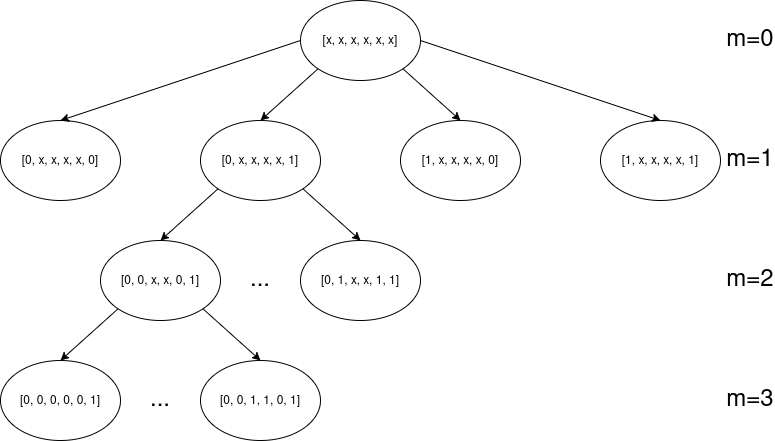
\includegraphics[scale=0.6]{Chapters/prn_search/branching_example.png}
    \caption{An example of the branching used in \citet{Mertens_1996} with
    $n = 6$ and where x represent unfixed values.}
    \label{prn_search:fig:1}
  \end{figure}

  When a symbol of the original sequence is complemented,
  the components of the autocorrelation can be decremented by, at most, 2. Based on
  that, a relaxation of $E_{min}$ can be proposed:\\
  \begin{equation}
    E_b = \sum_{k=1}^{n-1}max\{b_k, (|A'_k| - 2f_k)^2\} \leq E_{min}
  \end{equation}
  where $A'_k$ is the autocorrelation of an arbitrary sequence, $b_k = (n -
  k) \bmod 2$ the minimum possible value for $|A'_k|$ and $f_k$ the number of
  unfixed elements in $A'_k$ given by:
  \begin{equation}
    f_k = \left\{\begin{array}{ll}
        0 & k \geq N - m \\
        2(n - m - k) & n/2 \leq k < n - m\\
        n - 2m & k < n/2 \\
    \end{array}\right.
  \end{equation}

  where $n$ is the size of the sequence to search and $m$ the number of fixed
  elements at the ends of the sequence.\\

  If $E_b$ is greater than the best candidate for $E_{min}$ so far, that branch
  can be pruned reducing the amount of computation. With this algorithm,
  Mertens succesfully computed sequences up to length $n = 48$.\\

  This work was further improved by \citet{Packebusch_2016} combining bounds provided by different authors (Prestwich and
  Wiggenbrock) to create a new bound and  lowering the
  complexity to $O(1.729^n)$ obtaining sequences of length  $n= 66$. This
  record was broken by \citet{anatoli} by computing sequences up to length $n = 85$.\\

  \section{Our approach}

  To tackle the huge complexity encountered in the previous methods, a different
  approach was taken. Instead of dealing with the combinatorial explosion
  of all the possible binary sequences of length $n$, we decided to work with
  a smaller set consisting on all the possible sequences which can be
  constructed through the composition method with Legendre base sequences.\\

  This approach haves some pros and cons. First of all, the search space is
  reduced from $O(2^n)$ to $O(p^m)$ where $p*m = n$. This clearly means that
  the complexity grows slower than in previous works. In fact, the
  autocorrelation function can be optimized for sequences generated through the
  composition method as shown in a following chapter. \domingo {referencia el capitulo}\\

  The problem is that the possible lengths for the sequences are limited as $m$
  and $p$ are required to be coprime. Even though it means that
  these method cannot find optimal sequences for all lengths, the restriction is
  looser than the non-exhaustive methods. Apart from that, this method does not
  explore all possible permutations and it does not ensure to find a pseudonoise
  sequence if it exists. To sum up, this method is a good way to construct useful sequences but should not
  be used to prove the non existence of pseudonoise sequences for a given
  length.\\

  Given a base sequence of length $p$ and  shift sequences of length $m$ ,
  our program needs to find all the shift sequences that generate a composite
  sequence with a good autocorrelation.\\

  This means that the search space are all the posible permutations of the
  shift sequence, in other words, $p^m$ permutations. However, there are some
  relations between the different shift sequences that let us narrow the
  search space.\\

  For example, if a constant is added to every component of the shift sequence,
  a shifted version of the same sequence is obtained. This means that if only
   permutations that start with the same component are computed,
  then the whole search space would be covered as any other permutations would just
  be shifts of one permutation from the computed set. This optimization narrows
  our search space to $p^{(m-1)}$.\\

  Other optimization arises from the form of the shift sequences. In general,
  if the symbols are repeated often, they tend to generate higher
  autocorrelation spikes or periods inside the composite sequence. This
  concept can be easily expressed with the Hamming autocorrelation function:\\

  \begin{definition}[Hamming autocorrelation]
    Given a sequence $S$ of length $n$ and the  $shift$ function  defined at
    Equation \eqref{eq:3}, the Hamming autocorrelation is defined as:
      \begin{equation} \label{hamming:eq:1}
        HA(S)_{\tau} = \sum_{\tau = 0}^{n-1} HAComponent(S_{\tau}, shift(S, \tau)_{\tau})
      \end{equation}
    where $HAComponent$ is defined as:
      \begin{equation}
        HAComponent(c1, c2) = \left\{\begin{array}{lr}
            1  &  c1 = c2\\
            0  & \textnormal{otherwise} \\
        \end{array}\right.
      \end{equation}
  \end{definition}

  For our branch and bound algorithm, it is important to note that if a symbol
  that only appears once is substituted for another, the hamming
  autocorrelation won't get lower. This means that if a depth-in-first
  bounding of the nodes that have a hamming autocorrelation higher than the
  threshold (we mean, the maximum non trivial component) is performed,
  all nodes in that branch are ensured to have a higher hamming autocorrelation
  than the threshold.\\

  \begin{figure}[ht!]
    \begin{center}
      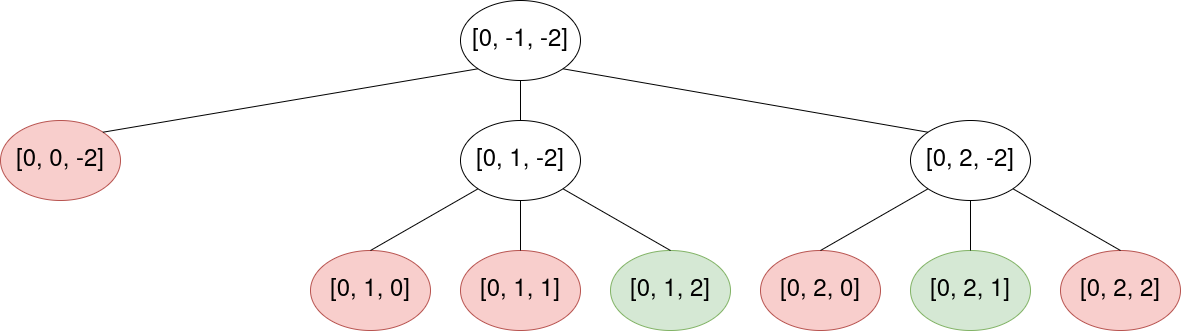
\includegraphics[scale=0.4]{Chapters/Implementation/Example_branch_bound.png}
    \end{center}
    \caption{An example of the branch and bound algorithm with a threshold for
    hamming autocorrelation of 1 and a base sequence of length 3. Red nodes
    represent prunes and green ones final nodes in which the
    autocorrelation is computed and checked. Negative values represent those
    that haven't been initialized yet.}
    \label{bb:fig:1}
  \end{figure}

  Some properties of the algorithm can be deduced from Figure \ref{bb:fig:1}.
  First of all, the number of autocorrelations computed can be reduced by a
  significant amount. However, the computation on each branch isn't balanced. This
  must be taken into account when the parallelism model is designed.


\chapter{Application development}

Before starting to code an application, the process has to be planned beforehand to guarantee that the project will be successful. Every different software project has different
characteristics that influence the decision on the methodology that should be followed.
Technologies, procedures, testing, time schedules, client meetings... All of
them must be taken into account to prevent extra work, bad quality software or
client dissatisfaction. In this chapter, we present the steps followed to design, construct and test an application to assist a designer to search for new binary sequences under certain requirements and to check their properties. Most of the information is mostly based on  \citet{Sommerville} and highly inspired in \citet{Mario_diaz}.

\section{Overall description}

  In this section we describe the  general idea behind the software project  and the requirements that needs to fulfill.
  \subsection{Project description}

  The main purpose of this project is to developed a software application to assist in the research of binary sequences with
  good correlation properties.The expected end-users are researchers but also designers for wireless communications systems such as radar, Wifi or GPS.\\

  The primary challenge is to understand the problema domain to create a software as useful as possible. Then, it is necessary to create an extensible program that assist in the   search  for new sequences to add to the existing scientific literature. Furthermore, a user has to  be able to  manage the sequences and  to check and compare their properties. As this process is computationally costly,  the software is expected to offer support for parallel computing.\\

 % \subsection{Product functions}

A summary of the functionalities that are expected from
  this software is provided.

  \begin{itemize}
    \item Perform computations in search for new sequences.\\
            \begin{itemize}
              \item Obtain real-time information of the computation process.
              \item Change dedicated resources to computation.
            \end{itemize}
    \item Manage the set of found sequences.
            \begin{itemize}
              \item Handle found sequences manually.
              \item Query by different sequence parameters .
              \item Plot sequence properties.
            \end{itemize}
  \end{itemize}

  \subsection{User classes and characteristics}

  Users of this project can be divided in two main groups:\\

  Researchers that will manage the search for new sequences, being capable of
  starting computations and modifying the database. These researchers are highly
  specialized personnel and are expected to be familiar with common abbreviations in
  the field, as well as knowing which parameters are more promising to get a
  successful computation.\\

  System administrators that will optimize the performance of the software according to the
  specifications of the system in which it is deployed. System administrators
  are specialized professionals which know how to run benchmarks, maximize
  performance and understand advanced concepts of parallel computing. 
  
  %They are  expected to be capable  of optimizing the software with a manual that explains the inner workings of the program in a technical jargon.\\

  In the real world, both roles may overlap in the same person.\\

  \subsection{Operating Environment}

  The computation module is expected to run in highly parallelized systems such
  as super-computers. Most researchers work with this kind of environments, so the software
  would be less competitive if it would not take full advantage of
  the capabilities of these systems.\\

  Taking this into account, the most common software installed in those environments should be
  targeted. This leads us to choose a Linux environment as most supercomputers
  run it.   We have chosen a Python interpreter as it is a popular language in the scientific
  community.\\


\section{Software requirements}

In this section we will introduce the software requirements of our project.

\subsection{Functional requirements}

The functional requirements of the project are shown in Figure
\ref{functional:fig}.


\begin{figure}[ht!]

  \begin{center}
    \begin{tabular}{||c | p{12cm}||}
      \hline
      Identifier & Description \\
      \hline
      \hline
      FR01 \label{FR01} & The researcher must be capable to set the base
      sequence to use for the search \\
      \hline
      FR02 \label{FR02} & The researcher must be capable to set the size
      of the shift sequence to use for the search\\
      \hline
      FR03 \label{FR03} & The researcher must be capable of setting the maximum
      autocorrelation he is interested in \\
      \hline
      FR04 \label{FR04} & The researcher must be capable to extract the
      results while the computation is still running (this doesn't mean that
      the data must be avalaible with a low latency)\\
      \hline
      FR05 \label{FR05} & The system administrator must be capable of changing
      the resources assigned to the program\\
      \hline
      FR06 \label{FR06} & The system must provide an interface that shows
      the progress of the computation (again, there's no need for low latency
      as it would conflict with \hyperref[NFR01]{NFR01})\\
      \hline
      FR07 \label{FR07} & Once established the parameters, the software must
      run without needing supervision of any user \\
      \hline
      FR08 \label{FR08} & The parameters of the load balancer must be editable
      by the system admin (as different machines might need different values)
      \\
      \hline
      FR09 \label{FR09} & An administrator must be capable of managing
      privileges for accesing the database and running computations\\
      \hline
      FR10 \label{FR10} & The system must provide a way to queue different
      searches to compute in succesion\\
      \hline
    \end{tabular}
  \end{center}

  \caption{Functional requierements}
  \label{functional:fig}
\end{figure}

\subsection{Non-functional requirements}

The non-functional requirements of the project are shown in Figure
\ref{non_functional:fig}.

\begin{figure}[ht!]

  \begin{center}

    \begin{tabular}{||c | c | p{7cm} | c||}

    \hline
    Identifier & Type  & Description & Relevance\\
    \hline
    \hline
    NFR01 \label{NFR01} & Performance & As we are searching for sequences in a
    huge space, speed is a top priority to continue with the research &
    Very high\\
    \hline
    NFR02 \label{NFR02} & Compability & As we are deploying our project in a
    research enviroment with different arquitectures, we must try to make it as
    compatible as posible in the case it must be changed to another node &
    Medium \\
    \hline
    NFR03 \label{NFR03} & Usability & This software is expected to be used by
    specialized researchers and it isn't an interactive application, so the
    time spent dealing with the application by users is low. Interface
    shouldn't be a priority & Very low \\
    \hline
    NFR04 \label{NFR04} & Arquitecture & The program must take full advantage
    of the capabilities of a supercomputer, in particular the high
    degree of parallelization of the system & High\\
    \hline
    NFR05 \label{NFR05} & Robustness & The program must not produce errors.
    Corruption of data, miscalculations or precision errors must not be
    tolerated as it would screw up the whole result & Very high \\
    \hline
    NFR06 \label{NFR06} & Robustness & The program cannot have memory leaks.
    It's expected to run for a long time and a memory leak can cause a crash.
    It can be fixed by restarting memory leaked threads without affecting the
    end result & Medium \\
    \hline
    NFR07 \label{NFR07} & Extensibility & Since the program is used as part of
    a research, we need the parts of the software to be reusable in case the
    research shows a new posible use for the project as part of a new
    development & Medium \\
    \hline
    NFR08 \label{NFR08} & Data availability & The availability of the data
    isn't a main concern as the project doesn't aim to be an interactive
    platform & Low \\
    \hline
    NFR09 \label{NFR09} & Robustness & The persistence layer must be robust
    enough to avoid data loses since it is costly to produce & High \\
    \hline

    \end{tabular}

  \end{center}

  \caption{Non-functional requirements}
  \label{non_functional:fig}
\end{figure}

\subsection{User interface requirements}

UI design is an important topic of software engineering as the success of a
project is related directly to the users experience and how they relate to the
software.\\

First of all, note that the users are supposed to be experienced in the use of
computers, so a complex UI shouldn't be a problem. In this casse, even though
the easier the better, our development has a huge constraint on UI design that
should be taken into account: the special type of OS we are working with.\\

As we are working with supercomputers, we can encounter a minimalist enviroment
with no graphical desktop. For this reason, we should focus on a command line
based application with 2 different main sections:\\
\begin{itemize}
  \item Application launcher (resource allocation, parallelism model, etc.)
  \item Runtime interaction with the system (tasks management, database
  queries, etc.)
\end{itemize}

As most supercomputers run UNIX-based systems, our application should follow
the POSIX\cite{POSIX_arguments} standard on the way it treats arguments.
It should follow conventions such as the use of flags such as --help or
--verbose and providing a man page.\\

It will also provide a way to store the configuration of the system in case
the application must be restarted quickly (mainly platform specific
configuration such as parameters of the load balancer). \\


\section{Agile development}

    One of the most important tasks to do before starting a project is deciding
    which project management model to follow.\\

    In our case, this project is going to avoid a waterfall model, even though it is the taught model in branches  not focused
    in software engineering. In this case  agile development techniques adapted better to
    our problem for several reasons:
    \begin{itemize}
      \item The client is an active part of the project. This means that
      a lot of feedback can be obtained during development and issues can be fixed earlier in the development cycle.
      \item As this project is being developed in the middle of a health crisis,
      the availability of project resources cannot be predicted. This means
      that having a rigid schedule planned too ahead of time would not  be
      useful.
    \end{itemize}

    \subsection{Role definition}

    Two different roles have been defined:
    \begin{itemize}
      \item Developer, which will design, program, verify and manage the
      software project.
      %In this case, this person corresponds to the author of this report (Juan Toca).
      \item Client, which will provide the requirements for the project, as well
      as validating each iteration.
      % In this case, this person corresponds to  the director of this project (Domingo Pérez).
    \end{itemize}

    \subsection{Iterations}

      In this subsection we will discuss how the development iterations went.
      A convention is that when we say a C function, we are referring to a Cython
      code without CPython code, in other words, functions that do not call the
      Python interpreter. The reader can refer to Chapter \ref{chap:tech_choices}
      in case more information on the technologies mentioned in this
      section is needed.

      \subsubsection{Iteration 1: Composite autocorrelation}

      In this iteration, the development was focused on developing an efficient
      way of computing the autocorrelation function of a base sequence with a
      given shift sequence. 3 versions were developed:
      \begin{itemize}
        \item A pure C function that given the autocorrelation of the base
        sequence and the shift sequence computes the autocorrelation.
        \item A wrapper Python function for the previous function which
        computes the autocorrelation of the given base sequence and passes it
        to the C function.
        \item A pure C function which checks if the maximum component of the
        composite autocorrelation exceeds the threshold provided.
      \end{itemize}

      The two first functions are not  part of the actual exhaustive search
      algorithm, but will be useful if properties have to be checked when
      retrieving the results from the database. \\

      The test process consisted in checking that the python wrapper provided
      the same results as a naive implementation of the algorithm based in
      the convolution theorem (see Section \ref{section:impl:convolution}). From
      that, the third function was tested against the first one.\\

      At first, C functions with fused types were developed. Although it
      favors extensibility, the compiler presented errors related with
      fused types. Finally  it was decided to drop support for fused types
      as it was only expected to work with integers of 32 bits.\\

      \subsubsection{Iteration 2: Branch and bound algorithm}

      In this iteration we focused on a single threaded C implementation of the
      branch and bound algorithm. This function receives a threshold of the
      maximum autocorrelation the user is interested in, the maximum Hamming
      autocorrelation for the prune part of the algorithm and the base sequence
      to use.\\

      For this purpose, a C implementation of the maximum Hamming
      autocorrelation was developed and an implementation of Legendre sequences
      to be used as base sequences. More types of base sequences can be added
      in the future, but this one was explicitly asked by the client.\\

      The test designed for Legendre sequences exploits its flat
      autocorrelation to check the functions consistency. In the case of
      Hamming's autocorrelation, a test based on lower and upper
      bounds was designed.\\

      In the case of the branch and bound method, it will check that all the
      returned sequences satisfied the specified maximum autocorrelation.\\

      \subsubsection{Iteration 3: Parallelism}

      In this iteration, the main focus was to adapt the branch and bound algorithm
      to a parallel environment. To do that, the algorithm was incrementally
      improved. At first, branch and bound was only applied from a given depth and
      then it was decided to also apply it at the master's process level.\\

      In this case, this iteration was implemented in pure Python as it isn't
      critical code. Most runtime of slave processes will be spent in Cython
      functions and, for simplicity and reliability, it was decided to stick to
      Python.\\

      Tests in this iteration were made in a more manual fashion, running the
      code and checking that all results were coherent. Properly based test were not written in this iteration as the code was not mature enough.\\


      %This was done like this because the code being tested was completly impure and property
      %based tests wouldn't have a worthy coverage to effort relationship to
      %consider writing them.\\

      \subsubsection{Iteration 4: User Interface}

      In this iteration a suitable UI for the program was designed. To do so,
      two functionalities were implemented:
      \begin{itemize}
        \item Support for command line arguments to initialize tasks.
        \item A verbose mode to get statistics of the program.
      \end{itemize}

      Command line parameters complies to POSIX's standard and informs the
      user of possible errors in the input, while the verbose mode logs events
      with its corresponding times to debug the performance of the
      computation.\\

      Again, the testing of this module was purely manual because of all
      the IO involved. The user interface was shown and explained to the client
      to receive their approval.\\


\section{Verification}
  One of the most important parts of software development is verifying the
  software. In other words, checking that the semantics of the program built
  are the same as the intended ones. Testing since the early stages of a project
  is mandatory if a quality product and an efficient development
  process is to be accomplish.  A lot of time can be invested building a
  program to realize that it does not work or a fix might generate side effects that break other
  parts of the program and so on. 
  \subsection{Unit tests}

    Unit testing is the smallest piece of test suite in a project. There exist
    several approaches in the literature such as white box and black box
    testing. In our project, a mixed approach will be taken depending on the
    situation:

    \subsubsection{Property based tests}

    Property-based testing is a not so well known type of black box testing that
    is built around the idea of defining properties of functions instead of
    test cases. Originally implemented by the Haskell's library
    "QuickCheck"\cite{QuickCheck}, this paradigm excels at generating huge
    volumes of test cases with just some extra lines of code leading
    to improvements on the coverage over the search space. It is similar to the
    test automation explained by \citet{Sommerville} in Chapter 23, being the
    main difference that an oracle that predicts the value is not needed.
    Instead, just a property of the output is checked.\\

    A well implemented library(there are several of them, but in our case we are
    working with Hypothesis\cite{Hypothesis} since our project is built in
    Python) should be capable of applying most well practices of black box
    testing, such as edge cases, all pairs, etc.\\

    The main reason why this type of test suites were chosen is that all the
    properties are already defined in this document and can be used
    straightforward as test cases. In fact, as most of our functions
    are static and pure, the generator will be very simple so the
    tests will take full advantage of this paradigm. In Figure \ref{test_example},
    there is have an example of a property used for testing the codebase.\\

    \begin{figure}[ht!]
      \inputpython{Chapters/software_engineering/test_example.py}{0}{100}
      \caption{An example test for Corollary \ref{autocorrelation:coro:1}}
      \label{test_example}
    \end{figure}

    The problem with this paradigm is that it becomes way too complicated when
    the tested methods have side effects, IO, state machines, etc. As this
    kind of systems usually depend on complex rules to build the generator of
    all the components involved in this systems. For these kind of tests, we
    will rely on the old method of designing test cases by hand.\\

\section{Validation}

The validation process in this project depends highly in the iteration in which
we are:

\begin{itemize}
  \item In early iterations, the validation process might not be as important
  as the verification process. This reason is the core functionality of the
  program is an algorithm expressed in a technical manner with little margin
  to misinterpretations.
  \item In later iterations, the validation process gains weight in respect of
  the verification process as we dive into the UI design. In this case, there
  is more room for misunderstandings between client and developer so we must
  take this process into account.
\end{itemize}

Fortunately, we are working with an agile mindset so a validation
session can be performed often so that the developers introduce the new features to
our client. Then, he can try out the features and point out misunderstandings,
desired changes, etc.\\



\chapter{Technology choices}

  In this chapter, the technologies used in this project will be discussed
  as well as the reasons behind their adoption, pros and cons for this project
  and difficulties encountered during development.

  \section{SageMath}

SageMath\cite{Sage} is a Python mathematical suite used in research projects as
an enviroment for prototyping algorythms or math concepts in general.\\

In our case, it served as a junction point between a mathematician that is used
to express ideas in math expressions and a developer that is used to
understanding concepts by making them work. Apart from that, it was also
useful at generating some figures for this document.\\

For our use case, a way to share the notebooks through the cloud was needed.
We decided to work with a free version of CoCalc\cite{cocalc}. Even though it
served the purpose of sharing code without the need of using a repository,
I have to say that in terms of other services such as running the notebooks
was very dissapointing. For low demanding tasks it performs well, but for
bigger computations I had to copy the code and run it locally. In future
projects, I might try out the payed version (as it has tons of features)
or other alternatives.\\

  \section{CPython}

Python\footnote{https://python.org/} programming language is one of the most used
languages in scientific enviroments, as well as in system integration developments.\\

In our case, the usage of Python serves 2 different purposes:
\begin{itemize}
  \item It's the language the researchers are the most familiar with. This
  helps the project because it's finished, they can extend the
  software for their needs as they want.
  \item It's a language widely used. This means that it can expected support
  from a lot of platforms while having a high-quality bunch of libraries to work
  with.
\end{itemize}


In addition, the developer has a solid experience with the stack of
technologies around Python which shouldn't be understated. Furthermore, his
profiency in the language let's him explore more new concepts in the same time
such as MPI or the whole domain knowledge needed for this project.\\

  \section{Cython}

Python as a language comes in several implementations. CPython as the reference
implementation has its flaws, mainly its performance issues. As the
software being developed has performance constraints, using just the reference
implementation is not an option.\\

Fortunatly, there are alternative implementations such as Jython, IronPython,
etc. In our case, Cython\footnote{https://cython.org/}\cite{Cython_book} was the
chosen one as it provides a compiler to build C code with pseudo-Python. Python code
can be called from C functions an viceversa, proving useful when a system
with C level performance to operate with high-level Python libraries is needed.\\

To support the decision of using Cython for the critical parts of the code,
some benchmarks were developed to test the actual performance improvements. As
shown in figures \ref{Cython:fig:1} and \ref{Cython:fig:2}, Cython benefits
a lot from tasks that requires iterations, but when using vector arithmetics
with Numpy the performance impact drops. This is because behind the scenes
Numpy functions are just Python wrappers for C functions so the heavy
computation is done in C.\\

\begin{figure}[ht!]
  \begin{center}
    \begin{tabular}{l r r}
      CPython:  & 318.65 seg & 100.0 \% \\
      Cython:   & 12.64 seg  & 3.9 \%   \\
      C:        & 12.33 seg  & 3.8 \%   \\
    \end{tabular}
  \end{center}
  \caption{Results of a benchmark of a long iteration.}
  \label{Cython:fig:1}
\end{figure}

\begin{figure}[ht!]
  \begin{center}
    \begin{tabular}{l r r}
      CPython:            & 8.66 seg & 100.0 \% \\
      Cython unoptimized: & 8.64 seg & 099.7 \% \\
      Cython optimized:   & 8.26 seg & 095.3 \% \\
      Cython GSL:         & 8.24 seg & 095.1 \%
    \end{tabular}
  \end{center}

  \caption{Results of a benchmark of vector operations using
  Numpy\footnotemark  \ or
  GSL\footnotemark.}
  \label{Cython:fig:2}
\end{figure}

\footnotetext[5]{https://numpy.org/}
\footnotetext{https://gnu.org/software/gsl/}

One might think that, if vector operations are so efficient in CPython, it would
be simpler to just use Numpy methods to implement our algorithms (which was
indeed done in the general autocorrelation function with the algortyhm
based on the convolution theorem). The problem raises when it is needed to
access the Numpy array in an undefined way by the library and to code a loop to
compute a function (the composite autocorrelation for example).\\

Cython provides native support for Numpy arrays, letting us access them with a
C level performance. In fact, as it supports fused types (the equivalent to
templates in C++), functions that can work with diverse types
depending on the input arguments can be defined. Even though in our case it will
be skipped as it comes with extra headaches and only integers are needed for the
purposes of this project, it is a nice feature if it was needed to extend Sage to
fully support our research field.\\

One important thing to take into account when developing with Cython is that
C types allocated in the heap (Cython supports raw C vectors and data structures
from C++ std) doesn't have automatic memory management. This will make the
debugging tougher as it will be needed to look for memory leaks. In contrast,
Numpy arrays do support automatic memory management at the cost of the overhead
of type checking and reference counting.\\

  \section{PostgreSQL}

PostgreSQL\footnote{https://postgresql.org/} is an open-source relational
database supported in a highly varied range of enviroments. As such, there is no
dependency on a particular Linux distribution to deploy (for example, Oracle only
supports RedHat).\\

Even if the database isn't as fast as Oracle or other databases, our
application isn't constraint by IO (as the generation of values to store in the
database depends directly in a costly computation). In our case, a persistence
system that supports well our stack of technologies is preferred. As
PostgreSQL is designed to run Python code on its SQL code, it gives a lot
of flexibility in how our application can be designed.



\chapter{Implementation}
  In this chapter, we will introduce some specifications of the implementation
  of our solution.\\


  \section{General autocorrelation function}
    The autocorrelation function introduced in Equation \ref{eq:4} can be
    implemented in several ways:

      \subsection{Naive approach}
        The naive approach for the autocorrelation function consists in
        computing all the displacements of the sequence and then
        their correlation with the base sequence as shown in Figure
        \ref{naive_auto:fig:1}. Even though this algorythm it's simple and
        follows the mathematical definition, is too slow. We have to compute
        the correlation function for each component, leading us to a
        complexity of $O(n^{2})$ where n it the size of the sequence with a
        huge constant as we have to build the shifted sequence for each
        component.\\

        This constant can be improved if we avoid building the shifts (just
        using slices of the array), but the complexity would stay the same.

      \subsection{Circular convolution theorem}
        The other option is to step in the world of mathematical properties.
        Fortunatly, there exists the convolution theorem\cite{golomb_ref} that
        lets us express the autocorrelation function in terms of Fourier
        Transforms as:
        \begin{theorem}
          Given a sequence $S$ and the Discrete Fourier Transform($DFT$):
          \begin{equation}
            A(S) = DFT^{-1}[DFT\{S\} · DFT\{S\}^{*}]
          \end{equation}
          where $DFT\{S\}^{*}$ represents the complex conjugate of $DFT\{S\}$.
        \end{theorem}

        Notice that, using the Fast Fourier
        Transform\cite{fast_fourier_transform}, the complexity of this
        method lowers to $O(N log N)$. However, its constant is
        still high as we need to apply 2 FFT to the sequence and apply the
        complex conjugate. In fact, we need to keep in mind that Fourier
        Transforms works with complex components while the naive approach keeps
        using the same type of components which makes its constant even higher
        than the naive approach.

          \begin{figure}
            \inputpython{Chapters/Implementation/naive.py}{0}{100}
            \caption{An example implementation of the naive autocorrelation}
            \label{naive_auto:fig:1}
          \end{figure}

      \subsection{Specific solution for the composition method}

      If we were to use a general method for this computation, we would
      probably use the one based on Fourier Transforms because we will be
      dealing with long sequences that will compensate the big constant of
      this method.\\

      However, we are dealing with sequences with the special property of
      having been built through the composition method. This means that we
      might find a non general way of computing this autocorrelation with better
      computational characteristics.\\

      If we take advantage of Property \ref{composition:prop:1}, we can design
      an algorythm with interesting properties. First of all, the complexity
      function depends on the size of the shift sequence. Being $m$ the
      length of the shift sequence and $n$ the length of the composite
      sequence, the resulting algortyhm has a complexity of $O(nm)$. This means
      that when $m < log(n)$ this algorythm has a better complexity than the
      Fourier Transform's approach.\\

      In addition, this algorythm has a better constant. We just need to
      iterate once through the autocorrelation sequence. This method is more
      cache friendly too as the data source of the function is smaller and it
      doesn't need to use complex operations in binary sequences.\\

      But the biggest improvement in respect of the Fourier Transform is that
      the complexity of a partial result of size $p$ is $O(mp)$ while the
      convolution theorem requires $O(nlog(n))$ for a partial result. In
      practice this means that if we just want to check a certain property
      of the autocorrelation we have no need to compute the whole function.\\

      An example implementation of this algorythm is shown in Figure \ref{composite_auto:fig:1}.

      \begin{figure}[ht!]
        \inputpython{Chapters/Implementation/composite.py}{0}{100}
        \caption{The Cython implementation of the composite autocorrelation.
        Notice that we used branchless programming to improve performance.}
        \label{composite_auto:fig:1}
      \end{figure}

  \section{Single-threaded Branch and Bound}

  The theoretical approach for the Branch and Bound algorithm has already
  explained. In this section, we introduce the actual implementation we used
  in the project in Figure \ref{composite_auto:fig:1}.

  \begin{figure}[ht!]
    \inputpython{Chapters/Implementation/branch_and_bound.py}{0}{100}
    \caption{A Cython implementation of the branch and bound algorythm. Notice
    the amount of extra code to achive C performance.}
    \label{composite_auto:fig:1}
  \end{figure}


  \section{Parallelism model}

  For the parallelism of the project, we decided to work with MPI. This model
  was implemented in pure Python as there was no need for a high performance in
  this part of the software (as the time spent in this code is already
  minimal).\\

  However, we need a low latency assignation of tasks. If we did use shared
  memory, every node would need to access memory through the "slow"
  interconnection network. Instead, with MPI, we can make the proccesses to
  talk between them.\\

  For the purpose of this project, we are going to work with
  MPICH\cite{mpich} as the bindings of MPI4PY support it and it's
  the implementation of the cluster we are working with\cite{calderon}.\\

  In our particular problem, we decided to define a set of tasks to
  distribute between the different nodes. This tasks are subtrees from the
  search space with a given height that defines the size of the task. An
  example is show in Figure \ref{tasks:fig:1}. Notice that the tasks are
  completly unbalanced so a static scheduler wouldn't be efficient at all.\\


  \begin{figure}[ht!]
    \begin{center}
      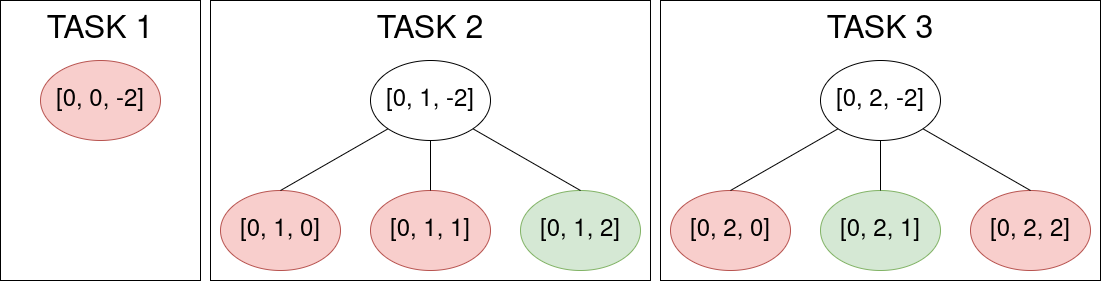
\includegraphics[scale=0.4]{Chapters/Implementation/Example_tasks.png}
    \end{center}
    \caption{An example distribution of tasks for the example at Figure
    \ref{bb:fig:1}.}
    \label{tasks:fig:1}
  \end{figure}

  This model is a good first version. However if we don't prune when assigning
  the tasks we will still have an exponential number of tasks (specifically,
  $n^{l-t}$ where $n$ is the length of the base sequence, $l$ the length of
  the shift sequence and $t$ the task size). This shouldn't be a problem if
  $t$ is close to $l$, but this will raise an issue with the task balancer as
  there wouldn't be enough tasks to balance the load.\\

  A second version of the algorithm applies the branch and bound algorythm in
  the master proccess to generate only tasks with good Hamming properties.
  This rules out all tasks that would instantly result in a bad
  autocorrelation and wouldn't generate any useful sequences. The code
  implementation is shown in Figures \ref{parallelism_example:fig:1} and
  \ref{parallelism_example:fig:2}.\\

  \begin{figure}[ht!]
    \inputpython{Chapters/Implementation/Example_parallelism_master.py}{0}{100}
    \caption{A Python implementation of the master proccess}
    \label{parallelism_example:fig:1}
  \end{figure}

  \begin{figure}[ht!]
    \inputpython{Chapters/Implementation/Example_parallelism_slave.py}{0}{100}
    \caption{A Python implementation of an slave proccess}
    \label{parallelism_example:fig:2}
  \end{figure}

  A third version (which we didn't implement because the second version was
  enough for our objective) could be done by using the Hamming as an
  heuristic to determine the size of the task. Instead of using a fixed size
  for the subtrees, we can give the tasks to the process at hand based on the
  Hamming autocorrelation of the root of the task.\\

  \section{UI implementation}

  Last but not least, we will briefly discuss the design of the User Interface.
  As expressed in the chapter of Sofware Engineering, our primary focus is
  its compatibility with command lines. For that, we used a POSIX compatible
  interface.\\

  First, we provided a --help option to list all the flags:
  \begin{lstlisting}
    $ python main.py --help
    usage: python main.py [option...]

    Options and arguments:
    -n : number of threads to use(must be compatible with your MPI enviroment)
         Defaults to the MPI configuration default

    -p : delay between polls in the master thread(higher values will make the
         slaves to wait more until the next task, lower values will increase
         CPU usage of master)

    -s : length of the base sequence(in this version must be a prime number to
         generate Legendre sequences. Other values have undefined behaviour)

    -l : length of shift sequences(this option must be coprime with value
         of s, other values have undefined behaviour)

    -t : size of the task for each thread(this option must be lower than the
         value provided by -l, other values have undefined behaviour)

    -h : maximum hamming autocorrelation allowed(this option must be a
         positive integer other values have undefined behaviour) Defaults to -l

    -c : maximum autocorrelation we are interested in(this option must be a
         positive integer other values have undefined behaviour) Defaults to
         the square root of (-l*-s)

    -v : verbose mode
  \end{lstlisting}

  Verbose mode logs which tasks have been assigned and at which time stamp, as
  well as logging the end of slave proccesses and the idle time of slaves:

  \begin{lstlisting}
    $ python main.py -s 5 -l 23 -t 20 -c 7 -h 3 -v
    2020-08-23 19:27:49 [1] : TASK_ASSIGNED [0, 0, 1] 9ms
    2020-08-23 19:27:49 [3] : TASK_ASSIGNED [0, 0, 3] 10ms
    2020-08-23 19:27:49 [5] : TASK_ASSIGNED [0, 0, 5] 6ms
    2020-08-23 19:27:49 [7] : TASK_ASSIGNED [0, 1, 1] 17ms
    2020-08-23 19:27:49 [6] : TASK_ASSIGNED [0, 1, 0] 3ms
    2020-08-23 19:27:49 [2] : TASK_ASSIGNED [0, 0, 2] 0ms
                            .
                            .
                            .
    2020-08-23 19:28:41 [1] : TASK_ASSIGNED [0, 5, 0] 0ms
    2020-08-23 19:28:42 [7] : TASK_ASSIGNED [0, 5, 3] 0ms
    2020-08-23 19:28:45 [1] : EXITED
    2020-08-23 19:28:45 [5] : TASK_ASSIGNED [0, 5, 2] 0ms
    2020-08-23 19:28:47 [2] : EXITED
    2020-08-23 19:28:48 [4] : TASK_ASSIGNED [0, 5, 4] 0ms
    2020-08-23 19:28:49 [6] : EXITED
    2020-08-23 19:28:52 [3] : EXITED
    2020-08-23 19:28:55 [5] : EXITED
    2020-08-23 19:28:56 [7] : EXITED
    2020-08-23 19:28:57 [4] : EXITED

  \end{lstlisting}

  Notice that, as we are using stdout, we can pipe the log to a file. The
  output format is designed in a way that eases the use of utilities such as
  awk to proccess the data of the program (one word message, well defined
  columns, etc.).\\

  Verbosity is completly optional and doesn't impact performance when inactive.
  It's particularly useful when tweaking the parameters to get the best
  configuration.\\


\chapter{Future work}

  Some work that must be still done is summarized in this chapter:
  \begin{itemize}
    \item The persistency module must be written with PostgreSQL as we are
    currently dumping the results in plain-text files.
    \item MPI usage can be farther improved if needed, nowadays we don't
    buffer new tasks in the nodes so the delay of the interconnection
    network haven't been mitigated.
    \item Because of a lack of time, I couldn't use Calderon to get some
    benchmarks for the parallelism model. This is a shame as some statistics
    on the complexity of our approach are a must to publish our results.
    \item Even if Domingo decided to stick with Legendre sequences to keep the
    program simple, it would probably be interesting to explore other kinds of
    base sequences.
    \item I should try to refactor the code to be more compatible with
    different versions of MPI as MPI4PY support all but I had to tweak my code
    to work in Calderon as I had used OpenMPI in my development process.
    \item My code isn't portable as Python's command conventions aren't
    standard. In Archlinux (my own system), the commands are python and python2
    while Debian (Calderon's system) uses python3 and python. As my main
    code wraps mpiexec, this is a pain to deal with.
    \item It would probably be useful to support config files as some
    parameters.
    for the command are common to all computations.
    \item I will have to consider if I really have to create a way to interact
    with the tasks and handle some kind of permissions as supercomputers seem
    to handle that for me.
    \item I will have to tidy up the code if Domingo wants to publish it as
    part of his investigation. Even though it's commented and it's readable,
    there are some parts that should be rewritten and optimized.
    \item We haven't expanded the literature yet so, at this stage, there's
    still some computations to be made.
  \end{itemize}

  This seems like a really long lists of TODOs. Keep in mind that this
  Bachelor thesis is a part of a research project that isn't yet finished. I
  think I've accomplish the goals that my director had for this thesis.

\chapter{Conclusions}

  The final results of the project can be sumarized as:
  \begin{itemize}
    \item I have acquired enough knowledge of the problem domain
    to be capable of helping to the researchers in their software needs.
    \item I have extended my knowledge in parallel computing by learning a
    new paradigm (Message Passing Parallelism).
    \item I have learned new tools (Cython and MPI) to fulfill the
    project needs.
    \item I have adapted my knowledge in functional programming and its
    robustness to develop the tests for this software.
    \item I have applied my knowledge in algorithmic complexity to make
    rational decisions on which is the best approach to a problem.
    \item I have overcome the limitations imposed by the current health crisis
    by changing my project management methodology to an agile development.
    \item I have learned how to manage a huge volume of scientific literature
    to carry out a research.
    \item I have started to work with a supercomputer to be capable of
    deploying this software and get actual results.
  \end{itemize}

  To conclude this report, I would like to provide some final thougts:
  \begin{itemize}

    \item After dealing with Cython, I have to say that I encountered many
    problems with the compiler. The GIL checker detected GIL usages in pure C
    code. The fused types are very cryptic. If I had to do another project
    with similar characteristics, I would probably write the core modules in
    C++ (To be able to use templates) and use Cython to create the
    bindings for Python.

    \item I recognize that I should have done some test in the supercomputer
    before starting the software engineering to check the availability
    of tools and the services that the supercomputer provides by itself.

    \item Even though I said I would try to develop a portable solution, as
    far I can tell from what I've worked so far with Calderon, i think that
    wasn't a realistic objective as the programs and tools available in each
    supercomputer seem to vary a lot.

    \item I have to be more methodic in my usage of GIT. Luckly I didn't need
    to do a rollback because my commits were huge and some of them in unstable
    states.

  \end{itemize}




\backmatter
% Indique aquí el fichero .bib que contenga su bibliografía.
\bibliography{refs}

\end{document}
